% !TeX root = thesis.tex
\documentclass{master_thesis}
\addbibresource{refs.bib}

\begin{document}

\section{Results}

\subsection{Comparing Results from Manual Audit and Automated Tests}

\info{RQ2: What kind of errors can be caught by running automated accessibility tests on a component library?}

A summarized table from all violations and passes in automated tests and issues found in the manual audit was created. In this table, the results have been reduced to counts that can be analyzed using statistical methods (see Appendix \ref{appendix:results-table}).

% summary of violations
The results show that addon-a11y did not report any violations for 27 (51\%) components out of 53 components after verifying the validity of these issues the number goes up to 31 (58\%) (see Figure \ref{fig:audit-failed}). On average the automated testing tool found 1 violation per component. The maximum number of violations reported for a single component was 7 and the maximum number of valid violations was 6.

% summary of passes
4 components out of 53 did not have any passed checks and 22 did not have any valid passed checks (see figure \ref{fig:audit-passed}). This means that the number of components with no valid passed checks changed from 4\%  to 42\% after manually validating the results. The highest number of passes were detected for \textit{Form} and \textit{Table} components (18). After validating the number of passes changed to 9 for Table and 7 for Form. The average number of passes for each component was 5 before and 2 after validating the results.

\begin{figure}[ht]
	\begin{subfigure}{0.45\textwidth}
	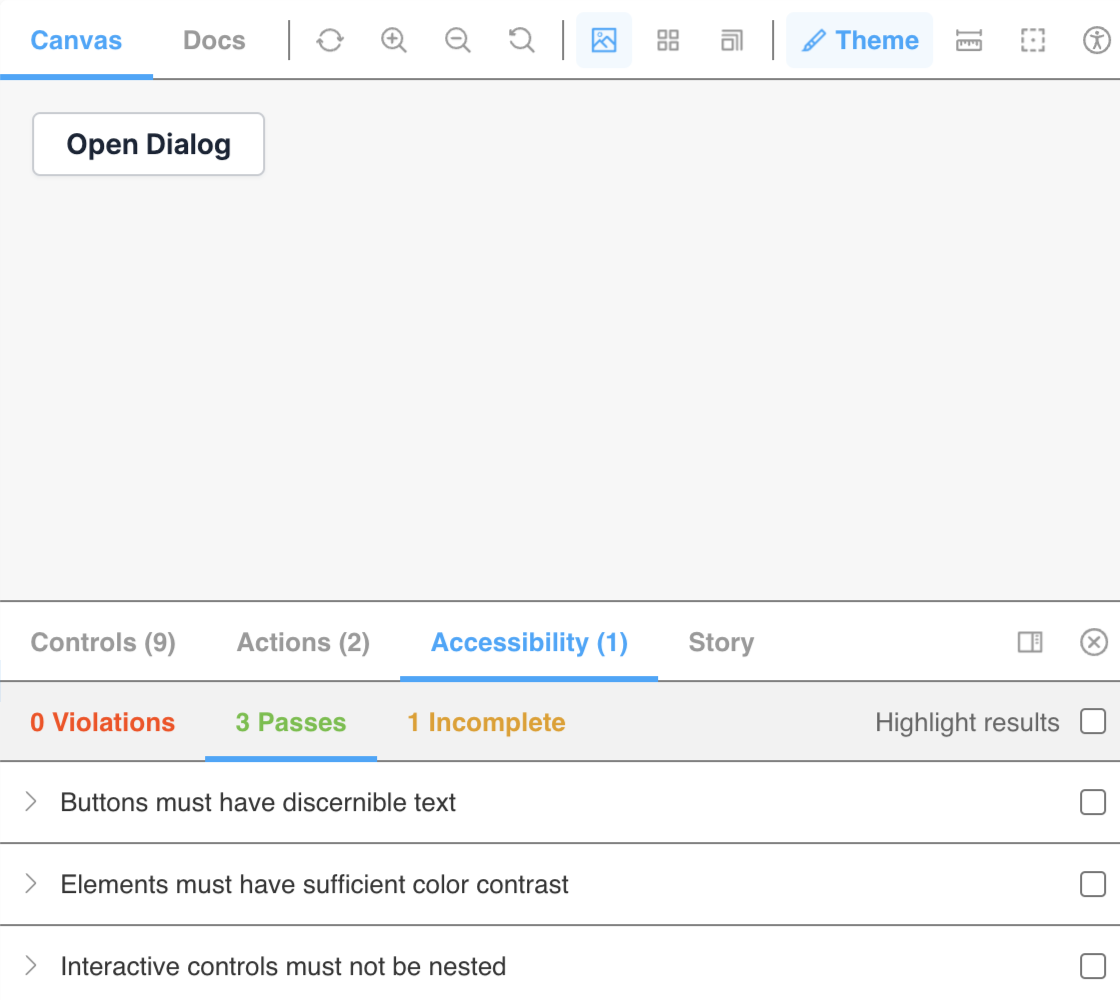
\includegraphics[width=\textwidth]{img/sb-button-trigger.png}
	\caption{Inital view of example. This is tested by addon-a11y.}
	\label{fig:sb-button-trigger-1}
	\end{subfigure}
	\hspace{0.05\textwidth}
	\begin{subfigure}{0.45\textwidth}
	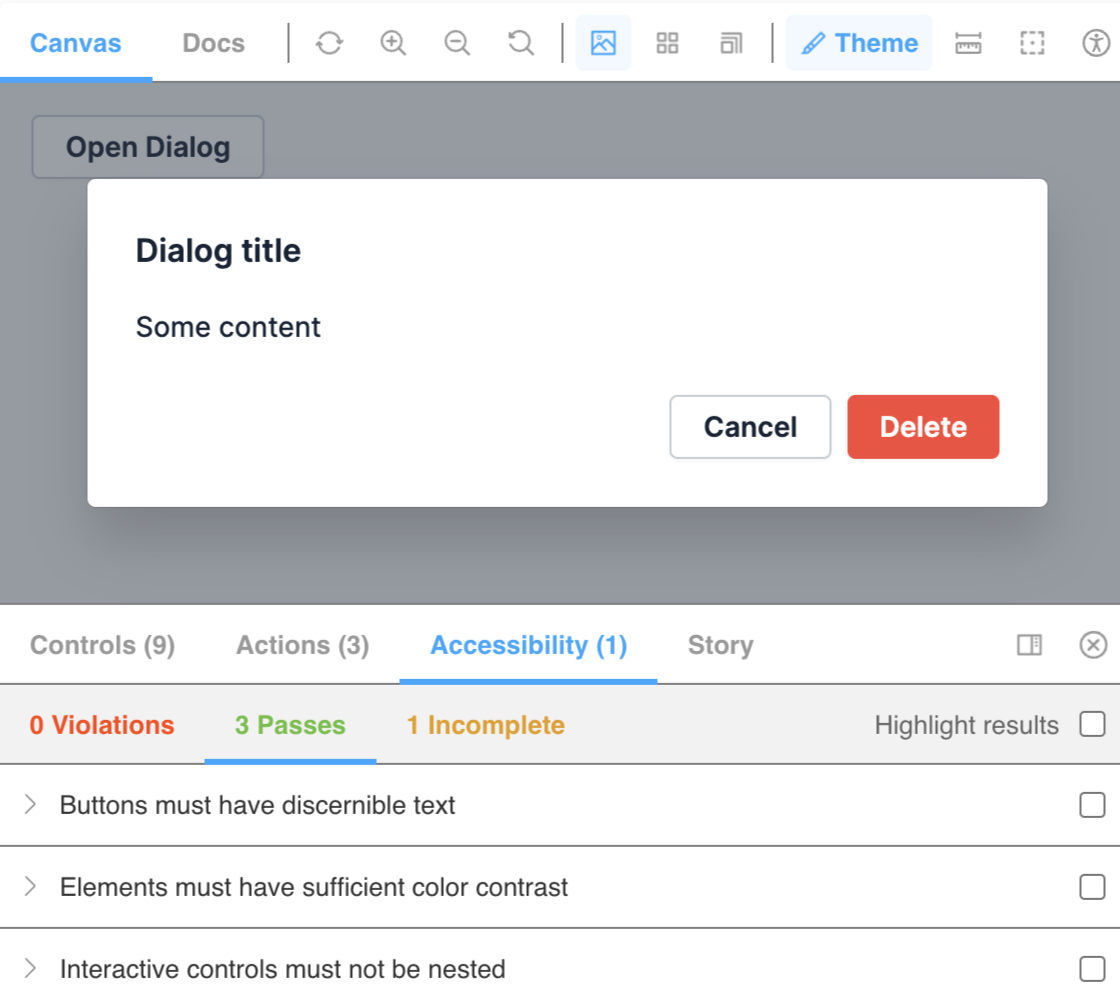
\includegraphics[width=\textwidth]{img/sb-button-trigger-open.png}
	\caption{Example after clicking the button and revealing the actual component.}
	\label{fig:sb-button-trigger-2}
	\end{subfigure}
\caption{Storybook example for Dialog component using button trigger}
\label{fig:sb-button-trigger}
\end{figure}

% summary of violations + passes
Looking at all the fails and passes gave a good overview of how many tests were run for each component. Out of 53 components that were tested, only 2 (4\%) did not get checked by addon-a11y at all, but some of these included false violations or passes. After validating the results the number of components not tested became 20 (38\%). This included components that become visible only when triggered by another element, like modals and popups that were displayed with a button as a trigger in the Storybook examples (see Figure \ref{fig:sb-button-trigger}). In total, there were 11 components with examples like that and they can be seen in Figure \ref{fig:audit-passed} starting from \textit{VideoOverlay} and ending with \textit{Coachmark}.

The remainder of the components that did not get tested by the addon included very simple components for spacing and visuals. These need further testing when they are being used in context to make sure that the visual info they are conveying is also included in text form. The results from manual testing did not reveal any further issues for 6 of these components. The components that have a trigger button in the example had the most additional issues. This is expected as due to the limitation of the examples the correct component was not evaluated by the tool.

Analyzing the validity of checks performed by addon-a11y further shows that from all passes and fails together a bit more than half are valid while 68\% of detected violations are correct and 51\% of passed checks were confirmed to be relevant (see Figure \ref{fig:checks-validity}).

\begin{figure}[ht]
	\centering
	\begin{subfigure}{0.3\textwidth}
	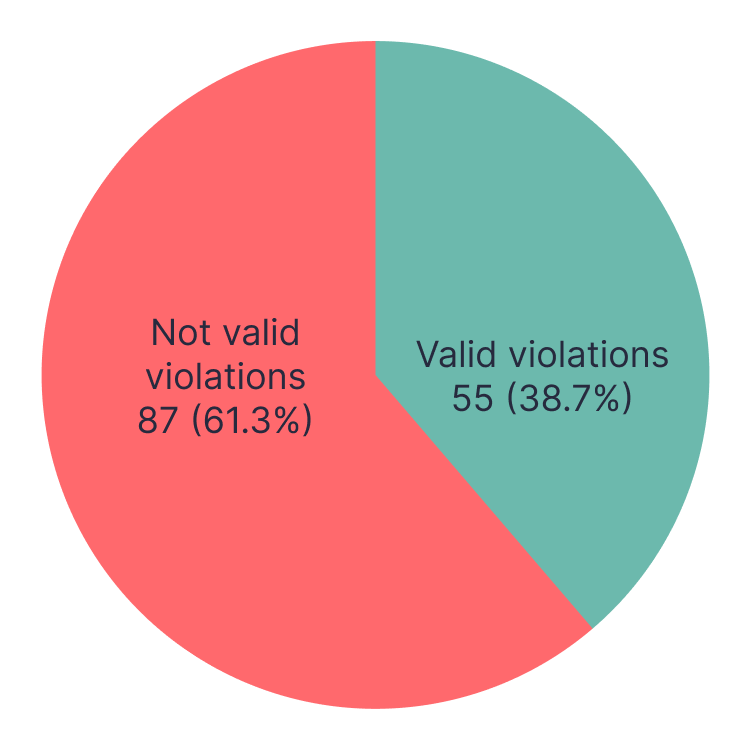
\includegraphics[width=\textwidth]{img/failed-tests.png}
	\caption{How many of the detected violations are valid?}
	\label{fig:checks-validity-failed}
	\end{subfigure}
	\hspace{0.03\textwidth}
	\begin{subfigure}{0.3\textwidth}
	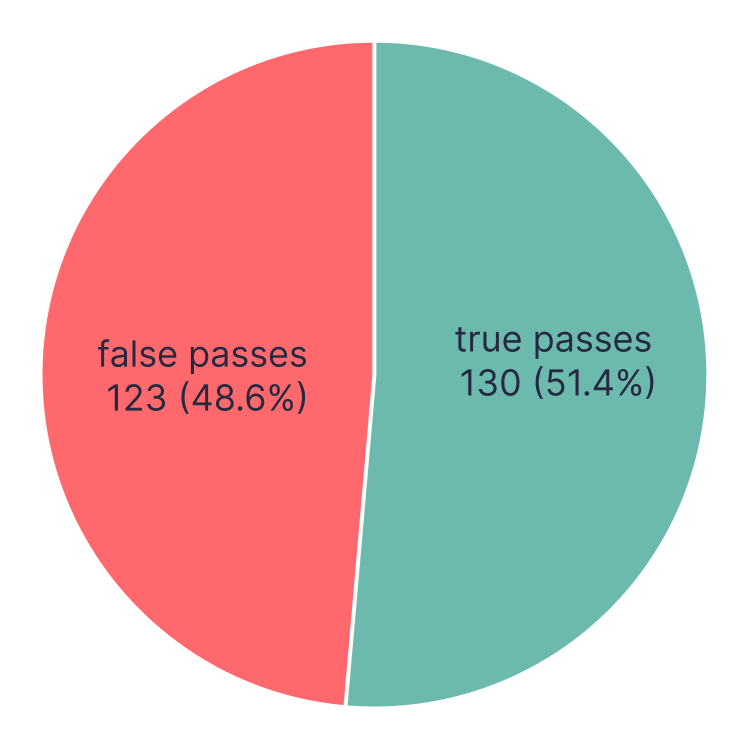
\includegraphics[width=\textwidth]{img/passed-tests.png}
	\caption{How many of the checks passed are valid?}
	\label{fig:checks-validity-passed}
	\end{subfigure}
	\hspace{0.03\textwidth}
	\begin{subfigure}{0.3\textwidth}
	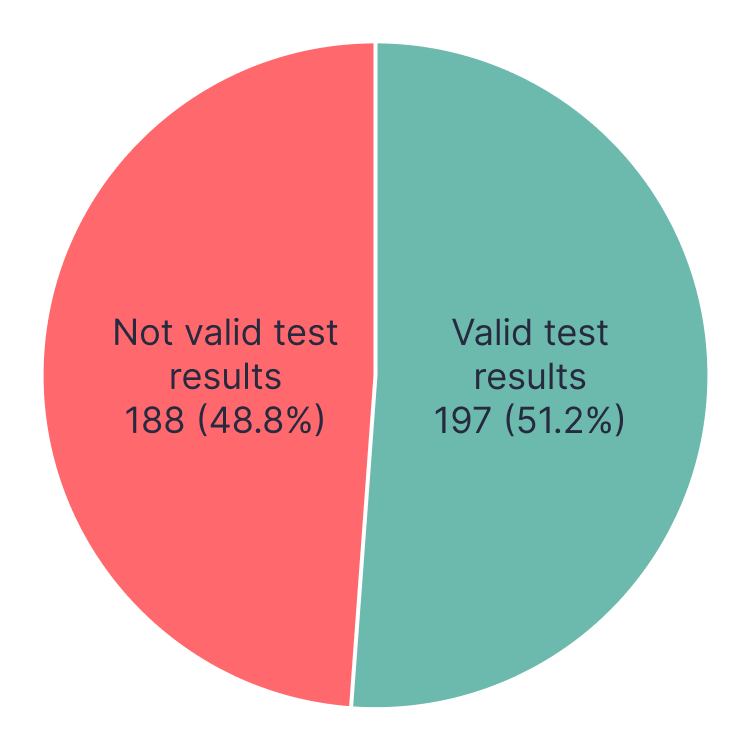
\includegraphics[width=\textwidth]{img/all-test-results.png}
	\caption{How many of all tests are valid?}
	\label{fig:checks-validity-all}
	\end{subfigure}
\caption{Valididty of tests performed by addon-a11y}
\label{fig:checks-validity}
\end{figure}

\textbf{RQ2}: "What kind of errors can be caught by running automated accessibility tests on a component library?" can be answered based on these results and the results from manually evaluating the same components. The \ac{wcag} Success Criterion, correct usage of \ac{waiaria} and other best practices that proved to be reliably testable in Pipedrive's component library are:

\begin{itemize}
	\item Success Criterion 1.1.1 Non-text Content
	% (https://www.w3.org/TR/WCAG21/#non-text-content)
	\begin{itemize}
		\item Images must have alternate text
	\end{itemize}

	\item Success Criterion 1.3.1 Info and Relationships
	% https://www.w3.org/TR/WCAG21/#info-and-relationships
	\begin{itemize}
		\item Certain ARIA roles must contain particular children: Required ARIA children role not present: cell, columnheader, gridcell, rowheader
	\end{itemize}

	\item Success Criterion 1.4.3 Contrast (Minimum)
	% (https://www.w3.org/TR/WCAG21/\#contrast-minimum)
	\item Success Criterion 1.4.6 Contrast (Enhanced)
	% (https://www.w3.org/TR/WCAG21/\#contrast-enhanced)
	\begin{itemize}
		\item Color contrast
	\end{itemize}

	\item Success Criterion 1.4.12 Text Spacing
	% (https://www.w3.org/TR/WCAG21/#text-spacing)
	\begin{itemize}
		\item Inline text spacing must be adjustable with custom stylesheets
	\end{itemize}

	\item Success Criterion 2.1.1 Keyboard
	\item Success Criterion 2.1.3 Keyboard (No Exception)
	% (https://www.w3.org/TR/WCAG21/#keyboard)
	% (https://www.w3.org/TR/WCAG21/#keyboard-no-exception)
	\begin{itemize}
		\item Scrollable region must have keyboard access
	\end{itemize}

	\item Success Criterion 2.4.4 Link Purpose (In Context)
	\item Success Criterion 2.4.9 Link Purpose (Link Only)
	% (https://www.w3.org/TR/WCAG21/#link-purpose-in-context)
	% (https://www.w3.org/TR/WCAG21/#link-purpose-link-only)
	\begin{itemize}
		\item Links with the same name must have a similar purpose
		\item Links must have discernible text
	\end{itemize}

	\item Success Criterion 4.1.1 Parsing
	% (https://www.w3.org/TR/WCAG21/#parsing)
	\begin{itemize}
		\item IDs used in ARIA and labels must be unique
	\end{itemize}

	\item Success Criterion 4.1.2 Name, Role, Value
	% (https://www.w3.org/TR/WCAG21/\#name-role-value)
	\begin{itemize}
		\item Buttons must have discernible text
		\item Form elements must have labels
		\item Form field must not have multiple label elements
		\item Form elements should have a visible label
		\item ARIA input fields must have an accessible name
		\item ARIA roles used must conform to valid values
		\item ARIA commands must have an accessible name
		\item Interactive controls must not be nested
	\end{itemize}

	\item Correct usage of WAI-ARIA
	% (https://www.w3.org/TR/wai-aria-1.1/#usage)
	\begin{itemize}
		\item ARIA attributes must conform to valid values
		\item ARIA attributes must conform to valid names
		\item Elements must only use allowed ARIA attributes
		\item Required ARIA attributes must be provided
	\end{itemize}

	\item Best Practices Rules
	\begin{itemize}
		\item ARIA role should be appropriate for the element
		\item Elements should not have tab index greater than zero
		\item Alternative text of images should not be repeated as text
		\item Headings should not be empty
		\item Heading levels should only increase by one
	\end{itemize}
\end{itemize}

There might be other \ac{wcag} Success Criteria that the tool is also capable of testing, but that just was not represented by this certain component and examples. The most common valid test result was color contrast. 45,1\% of all violations and passes were tested for contrast.

From the additional issues found in the manual audit, it would appear that the following issues should be manually tested in most cases:
\begin{itemize}
	\item Focus states
	\item Navigating by using a keyboard
	\item Navigating and interacting by using a screen reader
	\item Recognizable color differences between semantically different variants of one component
	\item Images and if they should have alt text
	\item Svgs and if they should have an aria-label
\end{itemize}

% What could be improved in component examples to make them more testable
Inaccurate results and missed issues indicated problems with how the component examples have been written. The following things could be improved to improve the results of automated testing:
\begin{itemize}
	\item variants of components that are meant to be used on dark backgrounds should always be displayed on a dark background
	\item Examples where the component gets triggered by a button should be avoided when possible
	\item pseudo-classes (like hover, focus etc) of interactive elements should be displayed in examples
	\item Examples should be simple and display one component at a time to reduce the number of irrelevant tests being run
\end{itemize}

\review{Mari-Ell: Do you have a solution on how to get them tested as well? Somehow display them without the need of the trigger? - Test out play functions with Storybook 7 and the built-in test runner.}

\begin{figure}[ht]
	\begin{subfigure}{0.45\textwidth}
	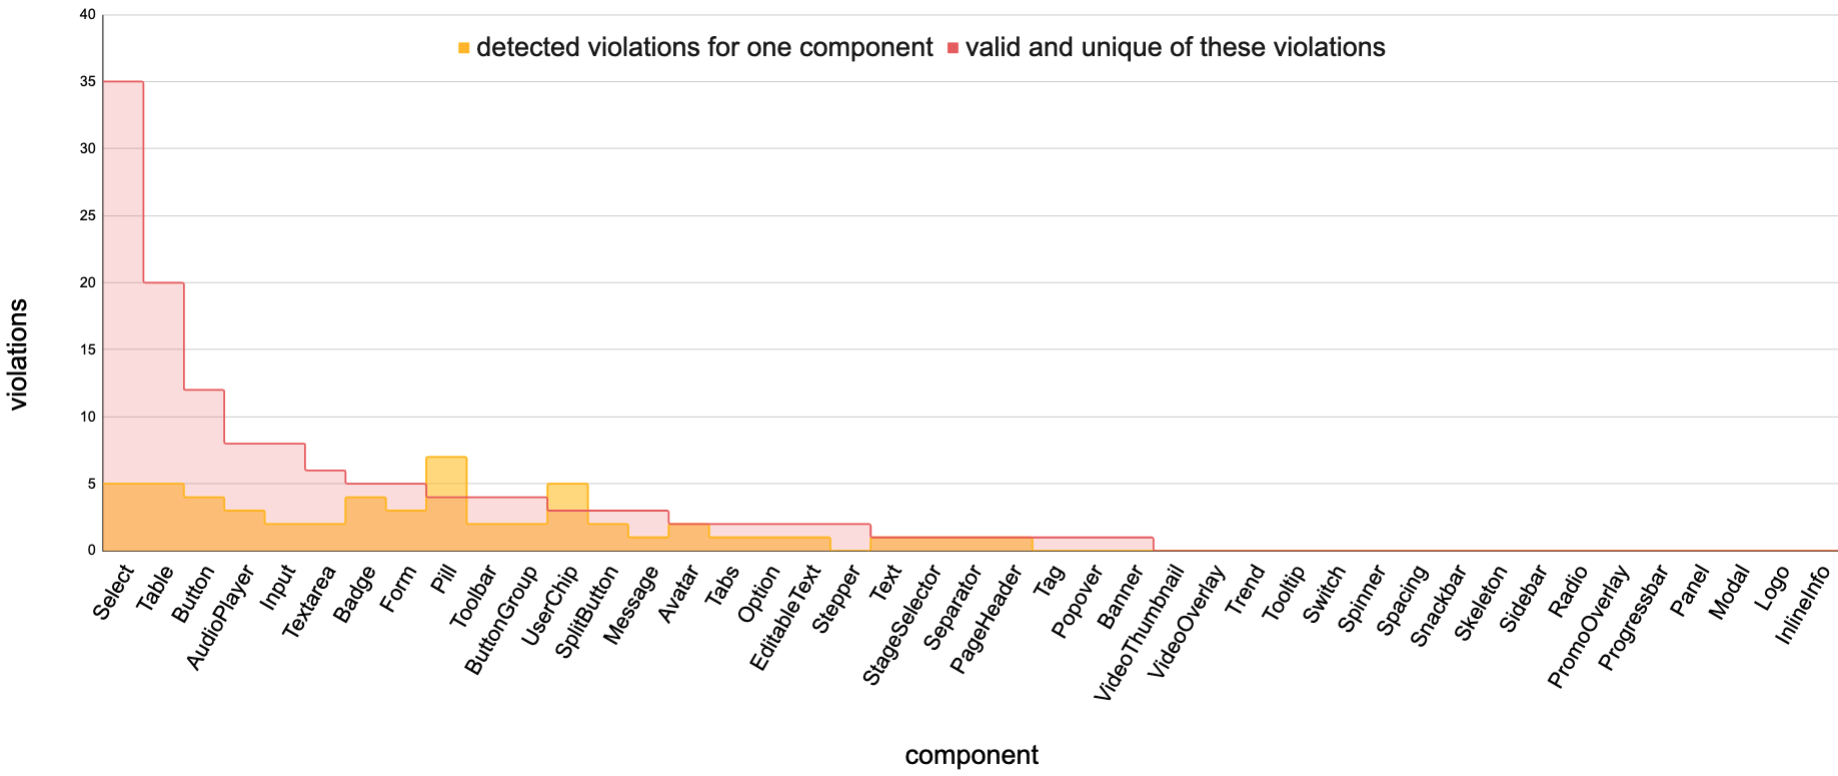
\includegraphics[height=0.9\textheight]{img/audit-failed.png}
	\caption{All violations reported by addon-a11y and how many of them are valid.}
	\label{fig:audit-failed}
	\end{subfigure}
	\hspace{0.05\textwidth}
	\begin{subfigure}{0.45\textwidth}
	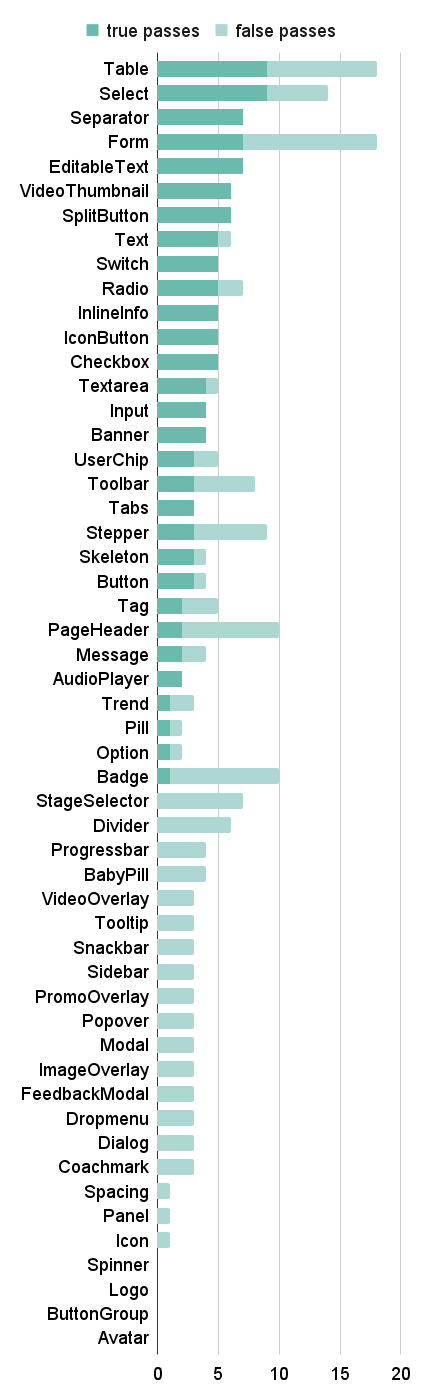
\includegraphics[height=0.9\textheight]{img/audit-passed.png}
	\caption{All passed checks reported by addon-a11y and how many of them are valid.}
	\label{fig:audit-passed}
	\end{subfigure}
\caption{All issues checked by addon-a11y}
\label{fig:audit-passed-failed}
\end{figure}

\subsection{How Much Was Compliance with WCAG 2.1 Improved?}

\info{RQ3: To what extent can integrating automated testing into a component library's development pipeline help improve its compliance with \ac{wcag}?  }
compare reports (beginning, after manual audit + now) + automated testing done in a good way can raise awareness about the importance of automated testing and with more awareness accessibility gets more priority. I also think that it is much more helpful in cases where these testing tools can be implemented from the start. make storybook examples that work for accessibility tests and research. It will help make dealing with accessibility issues easier, it seems like a big thing - no one really knows how much time is needed. daunting even.

\subsection{Limitations of Automated Accessibility Testing}
\info{RQ4: What are the biggest problems of integrating automated accessibility testing into a component library's development workflow?}
button issue, not possible to add to CI currently - easy to not notice
\todo{Follow up survey + reach out to devs I know have used addon-a11y}
The accessibility add-on in Storybook analyzes the examples that have been made for the component and unsuitable examples can cause false results. Like components triggered by a button described before. This is because the initial \ac{html} that the accessibility tests are being run on only has the button and the tests are not being run again after triggering the element. This could potentially be remedied with better examples.

The biggest limitation of this tool currently is that it can only be viewed in Storybook. To see the number of passes and fails you need to open the accessibility tab for each component. I looked into ways of automating this so that the same checks could be run on every change to the library and added to the \ac{ci} workflow. In the current version of Storybook, there is no easy way to do this, but it will become much easier in the next major version.

Upgrading our component library to that version would need some extra work to make it compatible, but I have tested out this solution on a test library, and it seems like it would be an improvement. Running the tests in \ac{ci} would ensure that they are run every time someone makes a change and not only when we choose to. We could also block changes that don't pass the required accessibility checks.

\todo{Reasons for automated check not being effective}

\end{document}